\documentclass[twoside]{book}

% Packages required by doxygen
\usepackage{calc}
\usepackage{doxygen}
\usepackage{graphicx}
\usepackage[utf8]{inputenc}
\usepackage{makeidx}
\usepackage{multicol}
\usepackage{multirow}
\usepackage{textcomp}
\usepackage[table]{xcolor}

% Font selection
\usepackage[T1]{fontenc}
\usepackage{mathptmx}
\usepackage[scaled=.90]{helvet}
\usepackage{courier}
\usepackage{amssymb}
\usepackage{sectsty}
\renewcommand{\familydefault}{\sfdefault}
\allsectionsfont{%
  \fontseries{bc}\selectfont%
  \color{darkgray}%
}
\renewcommand{\DoxyLabelFont}{%
  \fontseries{bc}\selectfont%
  \color{darkgray}%
}

% Page & text layout
\usepackage{geometry}
\geometry{%
  a4paper,%
  top=2.5cm,%
  bottom=2.5cm,%
  left=2.5cm,%
  right=2.5cm%
}
\tolerance=750
\hfuzz=15pt
\hbadness=750
\setlength{\emergencystretch}{15pt}
\setlength{\parindent}{0cm}
\setlength{\parskip}{0.2cm}
\makeatletter
\renewcommand{\paragraph}{%
  \@startsection{paragraph}{4}{0ex}{-1.0ex}{1.0ex}{%
    \normalfont\normalsize\bfseries\SS@parafont%
  }%
}
\renewcommand{\subparagraph}{%
  \@startsection{subparagraph}{5}{0ex}{-1.0ex}{1.0ex}{%
    \normalfont\normalsize\bfseries\SS@subparafont%
  }%
}
\makeatother

% Headers & footers
\usepackage{fancyhdr}
\pagestyle{fancyplain}
\fancyhead[LE]{\fancyplain{}{\bfseries\thepage}}
\fancyhead[CE]{\fancyplain{}{}}
\fancyhead[RE]{\fancyplain{}{\bfseries\leftmark}}
\fancyhead[LO]{\fancyplain{}{\bfseries\rightmark}}
\fancyhead[CO]{\fancyplain{}{}}
\fancyhead[RO]{\fancyplain{}{\bfseries\thepage}}
\fancyfoot[LE]{\fancyplain{}{}}
\fancyfoot[CE]{\fancyplain{}{}}
\fancyfoot[RE]{\fancyplain{}{\bfseries\scriptsize Generated on Thu Apr 24 2014 07\-:31\-:46 for L\-A\-B7 by Doxygen }}
\fancyfoot[LO]{\fancyplain{}{\bfseries\scriptsize Generated on Thu Apr 24 2014 07\-:31\-:46 for L\-A\-B7 by Doxygen }}
\fancyfoot[CO]{\fancyplain{}{}}
\fancyfoot[RO]{\fancyplain{}{}}
\renewcommand{\footrulewidth}{0.4pt}
\renewcommand{\chaptermark}[1]{%
  \markboth{#1}{}%
}
\renewcommand{\sectionmark}[1]{%
  \markright{\thesection\ #1}%
}

% Indices & bibliography
\usepackage{natbib}
\usepackage[titles]{tocloft}
\setcounter{tocdepth}{3}
\setcounter{secnumdepth}{5}
\makeindex

% Hyperlinks (required, but should be loaded last)
\usepackage{ifpdf}
\ifpdf
  \usepackage[pdftex,pagebackref=true]{hyperref}
\else
  \usepackage[ps2pdf,pagebackref=true]{hyperref}
\fi
\hypersetup{%
  colorlinks=true,%
  linkcolor=blue,%
  citecolor=blue,%
  unicode%
}

% Custom commands
\newcommand{\clearemptydoublepage}{%
  \newpage{\pagestyle{empty}\cleardoublepage}%
}


%===== C O N T E N T S =====

\begin{document}

% Titlepage & ToC
\hypersetup{pageanchor=false}
\pagenumbering{roman}
\begin{titlepage}
\vspace*{7cm}
\begin{center}%
{\Large L\-A\-B7 \\[1ex]\large 0.\-1 }\\
\vspace*{1cm}
{\large Generated by Doxygen 1.8.6}\\
\vspace*{0.5cm}
{\small Thu Apr 24 2014 07:31:46}\\
\end{center}
\end{titlepage}
\clearemptydoublepage
\tableofcontents
\clearemptydoublepage
\pagenumbering{arabic}
\hypersetup{pageanchor=true}

%--- Begin generated contents ---
\chapter{Dokumentacja zadania P\-A\-M\-S\-I L\-A\-B 7}
\label{index}\hypertarget{index}{}\begin{DoxyAuthor}{Author}
Justyna Klijewska 
\end{DoxyAuthor}
\begin{DoxyDate}{Date}
28.\-05.\-2014 
\end{DoxyDate}
\begin{DoxyVersion}{Version}
0.\-1 
\end{DoxyVersion}

\chapter{Class Index}
\section{Lista klas}
Tutaj znajdują się klasy, struktury, unie i interfejsy wraz z ich krótkimi opisami\-:\begin{DoxyCompactList}
\item\contentsline{section}{\hyperlink{class_tablica}{Tablica} }{\pageref{class_tablica}}{}
\item\contentsline{section}{\hyperlink{class_zegar}{Zegar} }{\pageref{class_zegar}}{}
\end{DoxyCompactList}

\chapter{File Index}
\section{File List}
Here is a list of all files with brief descriptions\-:\begin{DoxyCompactList}
\item\contentsline{section}{C\-:/\-Users/\-Klijek/\-Documents/\-Git\-Hub/\-Pamis02/\-L\-A\-B8/prj/\hyperlink{graf_8cpp}{graf.\-cpp} }{\pageref{graf_8cpp}}{}
\item\contentsline{section}{C\-:/\-Users/\-Klijek/\-Documents/\-Git\-Hub/\-Pamis02/\-L\-A\-B8/prj/\hyperlink{graf_8hpp}{graf.\-hpp} }{\pageref{graf_8hpp}}{}
\item\contentsline{section}{C\-:/\-Users/\-Klijek/\-Documents/\-Git\-Hub/\-Pamis02/\-L\-A\-B8/prj/\hyperlink{main_8cpp}{main.\-cpp} }{\pageref{main_8cpp}}{}
\end{DoxyCompactList}

\chapter{Class Documentation}
\hypertarget{class_b_s_t}{\section{B\-S\-T Class Reference}
\label{class_b_s_t}\index{B\-S\-T@{B\-S\-T}}
}


Klasa \hyperlink{class_b_s_t}{B\-S\-T}.  




{\ttfamily \#include $<$B\-S\-T.\-hpp$>$}

\subsection*{Public Member Functions}
\begin{DoxyCompactItemize}
\item 
\hyperlink{class_b_s_t_abc17123a0367c3b8ad0382eeb3ad3178}{B\-S\-T} ()
\begin{DoxyCompactList}\small\item\em Konstruktor \hyperlink{class_b_s_t}{B\-S\-T}. \end{DoxyCompactList}\item 
\hyperlink{class_b_s_t_aff9c7948fbba37844d2893b920ddc238}{$\sim$\-B\-S\-T} ()
\begin{DoxyCompactList}\small\item\em Destruktor \hyperlink{class_b_s_t}{B\-S\-T}. \end{DoxyCompactList}\item 
bool \hyperlink{class_b_s_t_a95a77762742b21d14b999f97e957b8b9}{Add\-Key} (int inkey)
\begin{DoxyCompactList}\small\item\em Metoda Add\-Key. \end{DoxyCompactList}\item 
\hyperlink{struct_node}{Node} $\ast$ \hyperlink{class_b_s_t_afdab435b1437c0dc9a99318670658883}{Take\-Key} (int inkey)
\begin{DoxyCompactList}\small\item\em Metoda Take\-Key. \end{DoxyCompactList}\item 
\hyperlink{struct_node}{Node} $\ast$ \hyperlink{class_b_s_t_a9fc8f734b86958c96a3b2896ac6117a3}{Delete\-Key} (int inkey)
\begin{DoxyCompactList}\small\item\em Metoda Delete\-Key. \end{DoxyCompactList}\item 
\hyperlink{struct_node}{Node} $\ast$ \hyperlink{class_b_s_t_abf32ad40eb28fd4dc67658173eb86e78}{next} (\hyperlink{struct_node}{Node} $\ast$n)
\begin{DoxyCompactList}\small\item\em Metoda next. \end{DoxyCompactList}\item 
\hyperlink{struct_node}{Node} $\ast$ \hyperlink{class_b_s_t_ac9741aaabbbf9da9bf179c8f8b2430e4}{prev} (\hyperlink{struct_node}{Node} $\ast$n)
\begin{DoxyCompactList}\small\item\em Metoda prev. \end{DoxyCompactList}\item 
\hyperlink{struct_node}{Node} $\ast$ \hyperlink{class_b_s_t_af2d2ab24cf760c680bad9a665e478e09}{max\-N} (\hyperlink{struct_node}{Node} $\ast$n)
\begin{DoxyCompactList}\small\item\em Metoda max\-N. \end{DoxyCompactList}\item 
\hyperlink{struct_node}{Node} $\ast$ \hyperlink{class_b_s_t_ad4cb87dd7e870ae8bb6a5ee335114fe2}{min\-N} (\hyperlink{struct_node}{Node} $\ast$n)
\begin{DoxyCompactList}\small\item\em Metoda min\-N. \end{DoxyCompactList}\item 
int \hyperlink{class_b_s_t_ad2655cdcbb1922a258339c97622632ad}{Size} ()
\begin{DoxyCompactList}\small\item\em Metoda Size,. \end{DoxyCompactList}\end{DoxyCompactItemize}


\subsection{Detailed Description}
Klasa \hyperlink{class_b_s_t}{B\-S\-T}. 

Klasa drzewa binarnego. Odpowiada za nizej opisane metody 

\subsection{Constructor \& Destructor Documentation}
\hypertarget{class_b_s_t_abc17123a0367c3b8ad0382eeb3ad3178}{\index{B\-S\-T@{B\-S\-T}!B\-S\-T@{B\-S\-T}}
\index{B\-S\-T@{B\-S\-T}!BST@{B\-S\-T}}
\subsubsection[{B\-S\-T}]{\setlength{\rightskip}{0pt plus 5cm}B\-S\-T\-::\-B\-S\-T (
\begin{DoxyParamCaption}
{}
\end{DoxyParamCaption}
)}}\label{class_b_s_t_abc17123a0367c3b8ad0382eeb3ad3178}


Konstruktor \hyperlink{class_b_s_t}{B\-S\-T}. 

Konstruktor drzewa binarnego \hyperlink{class_b_s_t}{B\-S\-T}. \hypertarget{class_b_s_t_aff9c7948fbba37844d2893b920ddc238}{\index{B\-S\-T@{B\-S\-T}!$\sim$\-B\-S\-T@{$\sim$\-B\-S\-T}}
\index{$\sim$\-B\-S\-T@{$\sim$\-B\-S\-T}!BST@{B\-S\-T}}
\subsubsection[{$\sim$\-B\-S\-T}]{\setlength{\rightskip}{0pt plus 5cm}B\-S\-T\-::$\sim$\-B\-S\-T (
\begin{DoxyParamCaption}
{}
\end{DoxyParamCaption}
)}}\label{class_b_s_t_aff9c7948fbba37844d2893b920ddc238}


Destruktor \hyperlink{class_b_s_t}{B\-S\-T}. 

Destruktor drzewa \hyperlink{class_b_s_t}{B\-S\-T} 

Here is the call graph for this function\-:




\subsection{Member Function Documentation}
\hypertarget{class_b_s_t_a95a77762742b21d14b999f97e957b8b9}{\index{B\-S\-T@{B\-S\-T}!Add\-Key@{Add\-Key}}
\index{Add\-Key@{Add\-Key}!BST@{B\-S\-T}}
\subsubsection[{Add\-Key}]{\setlength{\rightskip}{0pt plus 5cm}bool B\-S\-T\-::\-Add\-Key (
\begin{DoxyParamCaption}
\item[{int}]{inkey}
\end{DoxyParamCaption}
)}}\label{class_b_s_t_a95a77762742b21d14b999f97e957b8b9}


Metoda Add\-Key. 

Dodaje wartosc do naszego drzewa. Sprawdza, czy ma sie on znajdowac po lewej czy po prawej stronie (jak w zalozeniu drzewa). \hypertarget{class_b_s_t_a9fc8f734b86958c96a3b2896ac6117a3}{\index{B\-S\-T@{B\-S\-T}!Delete\-Key@{Delete\-Key}}
\index{Delete\-Key@{Delete\-Key}!BST@{B\-S\-T}}
\subsubsection[{Delete\-Key}]{\setlength{\rightskip}{0pt plus 5cm}{\bf Node} $\ast$ B\-S\-T\-::\-Delete\-Key (
\begin{DoxyParamCaption}
\item[{int}]{inkey}
\end{DoxyParamCaption}
)}}\label{class_b_s_t_a9fc8f734b86958c96a3b2896ac6117a3}


Metoda Delete\-Key. 

Usuwa wezel z drzewa. 

Here is the call graph for this function\-:




Here is the caller graph for this function\-:


\hypertarget{class_b_s_t_af2d2ab24cf760c680bad9a665e478e09}{\index{B\-S\-T@{B\-S\-T}!max\-N@{max\-N}}
\index{max\-N@{max\-N}!BST@{B\-S\-T}}
\subsubsection[{max\-N}]{\setlength{\rightskip}{0pt plus 5cm}{\bf Node} $\ast$ B\-S\-T\-::max\-N (
\begin{DoxyParamCaption}
\item[{{\bf Node} $\ast$}]{n}
\end{DoxyParamCaption}
)}}\label{class_b_s_t_af2d2ab24cf760c680bad9a665e478e09}


Metoda max\-N. 

Wyszukuje najwieksza wartosc wezla 

Here is the caller graph for this function\-:


\hypertarget{class_b_s_t_ad4cb87dd7e870ae8bb6a5ee335114fe2}{\index{B\-S\-T@{B\-S\-T}!min\-N@{min\-N}}
\index{min\-N@{min\-N}!BST@{B\-S\-T}}
\subsubsection[{min\-N}]{\setlength{\rightskip}{0pt plus 5cm}{\bf Node} $\ast$ B\-S\-T\-::min\-N (
\begin{DoxyParamCaption}
\item[{{\bf Node} $\ast$}]{n}
\end{DoxyParamCaption}
)}}\label{class_b_s_t_ad4cb87dd7e870ae8bb6a5ee335114fe2}


Metoda min\-N. 

Wyszukuje najmniejsza wartosc wezla 

Here is the caller graph for this function\-:


\hypertarget{class_b_s_t_abf32ad40eb28fd4dc67658173eb86e78}{\index{B\-S\-T@{B\-S\-T}!next@{next}}
\index{next@{next}!BST@{B\-S\-T}}
\subsubsection[{next}]{\setlength{\rightskip}{0pt plus 5cm}{\bf Node} $\ast$ B\-S\-T\-::next (
\begin{DoxyParamCaption}
\item[{{\bf Node} $\ast$}]{n}
\end{DoxyParamCaption}
)}}\label{class_b_s_t_abf32ad40eb28fd4dc67658173eb86e78}


Metoda next. 

Tworzenie nastepnika. 

Here is the call graph for this function\-:




Here is the caller graph for this function\-:


\hypertarget{class_b_s_t_ac9741aaabbbf9da9bf179c8f8b2430e4}{\index{B\-S\-T@{B\-S\-T}!prev@{prev}}
\index{prev@{prev}!BST@{B\-S\-T}}
\subsubsection[{prev}]{\setlength{\rightskip}{0pt plus 5cm}{\bf Node} $\ast$ B\-S\-T\-::prev (
\begin{DoxyParamCaption}
\item[{{\bf Node} $\ast$}]{n}
\end{DoxyParamCaption}
)}}\label{class_b_s_t_ac9741aaabbbf9da9bf179c8f8b2430e4}


Metoda prev. 

Tworzenie poprzednika. 

Here is the call graph for this function\-:




Here is the caller graph for this function\-:


\hypertarget{class_b_s_t_ad2655cdcbb1922a258339c97622632ad}{\index{B\-S\-T@{B\-S\-T}!Size@{Size}}
\index{Size@{Size}!BST@{B\-S\-T}}
\subsubsection[{Size}]{\setlength{\rightskip}{0pt plus 5cm}int B\-S\-T\-::\-Size (
\begin{DoxyParamCaption}
{}
\end{DoxyParamCaption}
)}}\label{class_b_s_t_ad2655cdcbb1922a258339c97622632ad}


Metoda Size,. 

zwraca ilo�� element�w w tablicy. \hypertarget{class_b_s_t_afdab435b1437c0dc9a99318670658883}{\index{B\-S\-T@{B\-S\-T}!Take\-Key@{Take\-Key}}
\index{Take\-Key@{Take\-Key}!BST@{B\-S\-T}}
\subsubsection[{Take\-Key}]{\setlength{\rightskip}{0pt plus 5cm}{\bf Node} $\ast$ B\-S\-T\-::\-Take\-Key (
\begin{DoxyParamCaption}
\item[{int}]{inkey}
\end{DoxyParamCaption}
)}}\label{class_b_s_t_afdab435b1437c0dc9a99318670658883}


Metoda Take\-Key. 

Zwraca wartosc przypisana do klucza. Tutaj mierzony jest tez czas 

Here is the caller graph for this function\-:




The documentation for this class was generated from the following files\-:\begin{DoxyCompactItemize}
\item 
C\-:/\-Users/\-Klijek/\-Desktop/\-L\-A\-B7/prj/B\-S\-T.\-hpp\item 
C\-:/\-Users/\-Klijek/\-Desktop/\-L\-A\-B7/prj/B\-S\-T.\-cpp\end{DoxyCompactItemize}

\hypertarget{struct_node}{\section{Node Struct Reference}
\label{struct_node}\index{Node@{Node}}
}


Struktura \hyperlink{struct_node}{Node}.  




{\ttfamily \#include $<$B\-S\-T.\-hpp$>$}



Collaboration diagram for Node\-:
\subsection*{Public Attributes}
\begin{DoxyCompactItemize}
\item 
\hypertarget{struct_node_ad8184598cdea70e4bbdfd76f2b0f9e85}{\hyperlink{struct_node}{Node} $\ast$ {\bfseries parent}}\label{struct_node_ad8184598cdea70e4bbdfd76f2b0f9e85}

\item 
\hypertarget{struct_node_a3ca572db95a35de41c87e70c3e8fb5a7}{\hyperlink{struct_node}{Node} $\ast$ {\bfseries left}}\label{struct_node_a3ca572db95a35de41c87e70c3e8fb5a7}

\item 
\hypertarget{struct_node_afe5916d969cd32f7de1e4ba15580c989}{\hyperlink{struct_node}{Node} $\ast$ {\bfseries right}}\label{struct_node_afe5916d969cd32f7de1e4ba15580c989}

\item 
\hypertarget{struct_node_a3020957813f200a9da836428aad2d8d7}{int {\bfseries key}}\label{struct_node_a3020957813f200a9da836428aad2d8d7}

\end{DoxyCompactItemize}


\subsection{Detailed Description}
Struktura \hyperlink{struct_node}{Node}. 

Struktura wezla. Mamy ty wezel 'parent', lewy oraz prawy (ktore sa tworzone wg danego algorytmu). 

The documentation for this struct was generated from the following file\-:\begin{DoxyCompactItemize}
\item 
C\-:/\-Users/\-Klijek/\-Desktop/\-L\-A\-B7/prj/B\-S\-T.\-hpp\end{DoxyCompactItemize}

\hypertarget{class_tab___aso}{\section{Dokumentacja szablonu klasy Tab\-\_\-\-Aso$<$ T\-\_\-\-K, T\-\_\-\-D $>$}
\label{class_tab___aso}\index{Tab\-\_\-\-Aso$<$ T\-\_\-\-K, T\-\_\-\-D $>$@{Tab\-\_\-\-Aso$<$ T\-\_\-\-K, T\-\_\-\-D $>$}}
}


Szablon klasy obs�uguj�cy tablice asocjacyjn� opart� na li�cie jednokierunkowej gdzie elementem listy jest struktura \hyperlink{struct_tab_aso_ele}{Tab\-Aso\-Ele}.  




{\ttfamily \#include $<$tab\-Aso.\-hpp$>$}

\subsection*{Metody publiczne}
\begin{DoxyCompactItemize}
\item 
\hyperlink{class_tab___aso_a8a4faa71b3dfbc4046e12bbd33a63f04}{Tab\-\_\-\-Aso} ()
\begin{DoxyCompactList}\small\item\em Kontruktor klasy \hyperlink{class_tab___aso}{Tab\-\_\-\-Aso}. \end{DoxyCompactList}\item 
\hyperlink{class_tab___aso_ab6601528f40554e7d288d780682ffd0c}{$\sim$\-Tab\-\_\-\-Aso} ()
\begin{DoxyCompactList}\small\item\em Destruktor klasy \hyperlink{class_tab___aso}{Tab\-\_\-\-Aso}. \end{DoxyCompactList}\item 
void \hyperlink{class_tab___aso_a13ed5efb41c50087eb40d15f7b858734}{Add\-Key} (T\-\_\-\-K inkey, T\-\_\-\-D indane)
\begin{DoxyCompactList}\small\item\em Metoda Add\-Key, dodaje par�, klucz -\/ warto�� do tablicy. \end{DoxyCompactList}\item 
void \hyperlink{class_tab___aso_aeb65c192e30a80ad78b4d16eede9a1f9}{Delete\-Key} (T\-\_\-\-K inkey)
\begin{DoxyCompactList}\small\item\em Metoda Delete\-Key, usuwa par�, klucz -\/ warto��. \end{DoxyCompactList}\item 
\hyperlink{struct_tab_aso_ele}{Tab\-Aso\-Ele}$<$ T\-\_\-\-K, T\-\_\-\-D $>$ $\ast$ \hyperlink{class_tab___aso_aa949662ff435df2b31ea91bc19c28baf}{Take\-Key} (T\-\_\-\-K inkey)
\begin{DoxyCompactList}\small\item\em Metoda Take\-Key, zwraca wska�nik na par� klucz -\/ warto��. \end{DoxyCompactList}\item 
bool \hyperlink{class_tab___aso_aa2fc214dc439b221c3d2805229c25b5d}{Is\-Empty} ()
\item 
void \hyperlink{class_tab___aso_aecbd56e2a0ff2239207e380eacd26580}{Change} (T\-\_\-\-K inkey, T\-\_\-\-D indane)
\begin{DoxyCompactList}\small\item\em Metoda Change zmienia warto�� dane na indane w podanym kluczu inkey. \end{DoxyCompactList}\item 
int \hyperlink{class_tab___aso_acd053d93f75de2d92a343a289f924b2b}{Size} ()
\begin{DoxyCompactList}\small\item\em Metoda Size, zwraca ilo�� element�w w tablicy. \end{DoxyCompactList}\item 
\hyperlink{struct_tab_aso_ele}{Tab\-Aso\-Ele}$<$ T\-\_\-\-K, T\-\_\-\-D $>$ $\ast$ \hyperlink{class_tab___aso_acd9f326d738bd2be240c8650c77388e3}{operator\mbox{[}$\,$\mbox{]}} (T\-\_\-\-K inkey)
\begin{DoxyCompactList}\small\item\em Przeci��enie operatora \mbox{[}\mbox{]}. \end{DoxyCompactList}\item 
\hyperlink{struct_tab_aso_ele}{Tab\-Aso\-Ele}$<$ T\-\_\-\-K, T\-\_\-\-D $>$ $\ast$ \hyperlink{class_tab___aso_a5cc0cab1284ef9c30200dec328e996ec}{operator\mbox{[}$\,$\mbox{]}} (int index)
\begin{DoxyCompactList}\small\item\em Przeci��enie operatora \mbox{[}\mbox{]}. \end{DoxyCompactList}\end{DoxyCompactItemize}


\subsection{Opis szczegółowy}
\subsubsection*{template$<$class T\-\_\-\-K, class T\-\_\-\-D$>$class Tab\-\_\-\-Aso$<$ T\-\_\-\-K, T\-\_\-\-D $>$}

Szablon klasy obs�uguj�cy tablice asocjacyjn� opart� na li�cie jednokierunkowej gdzie elementem listy jest struktura \hyperlink{struct_tab_aso_ele}{Tab\-Aso\-Ele}. 

T\-\_\-\-K -\/ Typ danych klucza T\-\_\-\-D -\/ Typ danych warto�ci 

Definicja w linii 33 pliku tab\-Aso.\-hpp.



\subsection{Dokumentacja konstruktora i destruktora}
\hypertarget{class_tab___aso_a8a4faa71b3dfbc4046e12bbd33a63f04}{\index{Tab\-\_\-\-Aso@{Tab\-\_\-\-Aso}!Tab\-\_\-\-Aso@{Tab\-\_\-\-Aso}}
\index{Tab\-\_\-\-Aso@{Tab\-\_\-\-Aso}!Tab_Aso@{Tab\-\_\-\-Aso}}
\subsubsection[{Tab\-\_\-\-Aso}]{\setlength{\rightskip}{0pt plus 5cm}template$<$class T\-\_\-\-K , class T\-\_\-\-D $>$ {\bf Tab\-\_\-\-Aso}$<$ T\-\_\-\-K, T\-\_\-\-D $>$\-::{\bf Tab\-\_\-\-Aso} (
\begin{DoxyParamCaption}
{}
\end{DoxyParamCaption}
)}}\label{class_tab___aso_a8a4faa71b3dfbc4046e12bbd33a63f04}


Kontruktor klasy \hyperlink{class_tab___aso}{Tab\-\_\-\-Aso}. 

Przy tworzeniu nowego obiektu tej klasy dodaje stra�nika kt�ry nie wskazuje na nic, natomiast koniec i pocz�tek listy wskazuje na stra�nika. 

Definicja w linii 63 pliku tab\-Aso.\-hpp.

\hypertarget{class_tab___aso_ab6601528f40554e7d288d780682ffd0c}{\index{Tab\-\_\-\-Aso@{Tab\-\_\-\-Aso}!$\sim$\-Tab\-\_\-\-Aso@{$\sim$\-Tab\-\_\-\-Aso}}
\index{$\sim$\-Tab\-\_\-\-Aso@{$\sim$\-Tab\-\_\-\-Aso}!Tab_Aso@{Tab\-\_\-\-Aso}}
\subsubsection[{$\sim$\-Tab\-\_\-\-Aso}]{\setlength{\rightskip}{0pt plus 5cm}template$<$class T\-\_\-\-K , class T\-\_\-\-D $>$ {\bf Tab\-\_\-\-Aso}$<$ T\-\_\-\-K, T\-\_\-\-D $>$\-::$\sim${\bf Tab\-\_\-\-Aso} (
\begin{DoxyParamCaption}
{}
\end{DoxyParamCaption}
)}}\label{class_tab___aso_ab6601528f40554e7d288d780682ffd0c}


Destruktor klasy \hyperlink{class_tab___aso}{Tab\-\_\-\-Aso}. 



Definicja w linii 78 pliku tab\-Aso.\-hpp.



\subsection{Dokumentacja funkcji składowych}
\hypertarget{class_tab___aso_a13ed5efb41c50087eb40d15f7b858734}{\index{Tab\-\_\-\-Aso@{Tab\-\_\-\-Aso}!Add\-Key@{Add\-Key}}
\index{Add\-Key@{Add\-Key}!Tab_Aso@{Tab\-\_\-\-Aso}}
\subsubsection[{Add\-Key}]{\setlength{\rightskip}{0pt plus 5cm}template$<$class T\-\_\-\-K , class T\-\_\-\-D $>$ void {\bf Tab\-\_\-\-Aso}$<$ T\-\_\-\-K, T\-\_\-\-D $>$\-::Add\-Key (
\begin{DoxyParamCaption}
\item[{T\-\_\-\-K}]{inkey, }
\item[{T\-\_\-\-D}]{indane}
\end{DoxyParamCaption}
)}}\label{class_tab___aso_a13ed5efb41c50087eb40d15f7b858734}


Metoda Add\-Key, dodaje par�, klucz -\/ warto�� do tablicy. 

key -\/ klucz dane -\/ warto�� 

Definicja w linii 95 pliku tab\-Aso.\-hpp.



Oto graf wywoływań tej funkcji\-:


\hypertarget{class_tab___aso_aecbd56e2a0ff2239207e380eacd26580}{\index{Tab\-\_\-\-Aso@{Tab\-\_\-\-Aso}!Change@{Change}}
\index{Change@{Change}!Tab_Aso@{Tab\-\_\-\-Aso}}
\subsubsection[{Change}]{\setlength{\rightskip}{0pt plus 5cm}template$<$class T\-\_\-\-K , class T\-\_\-\-D $>$ void {\bf Tab\-\_\-\-Aso}$<$ T\-\_\-\-K, T\-\_\-\-D $>$\-::Change (
\begin{DoxyParamCaption}
\item[{T\-\_\-\-K}]{inkey, }
\item[{T\-\_\-\-D}]{indane}
\end{DoxyParamCaption}
)}}\label{class_tab___aso_aecbd56e2a0ff2239207e380eacd26580}


Metoda Change zmienia warto�� dane na indane w podanym kluczu inkey. 



Definicja w linii 187 pliku tab\-Aso.\-hpp.



Oto graf wywoływań tej funkcji\-:


\hypertarget{class_tab___aso_aeb65c192e30a80ad78b4d16eede9a1f9}{\index{Tab\-\_\-\-Aso@{Tab\-\_\-\-Aso}!Delete\-Key@{Delete\-Key}}
\index{Delete\-Key@{Delete\-Key}!Tab_Aso@{Tab\-\_\-\-Aso}}
\subsubsection[{Delete\-Key}]{\setlength{\rightskip}{0pt plus 5cm}template$<$class T\-\_\-\-K , class T\-\_\-\-D $>$ void {\bf Tab\-\_\-\-Aso}$<$ T\-\_\-\-K, T\-\_\-\-D $>$\-::Delete\-Key (
\begin{DoxyParamCaption}
\item[{T\-\_\-\-K}]{inkey}
\end{DoxyParamCaption}
)}}\label{class_tab___aso_aeb65c192e30a80ad78b4d16eede9a1f9}


Metoda Delete\-Key, usuwa par�, klucz -\/ warto��. 

key -\/ klucz 

Definicja w linii 116 pliku tab\-Aso.\-hpp.



Oto graf wywoływań tej funkcji\-:


\hypertarget{class_tab___aso_aa2fc214dc439b221c3d2805229c25b5d}{\index{Tab\-\_\-\-Aso@{Tab\-\_\-\-Aso}!Is\-Empty@{Is\-Empty}}
\index{Is\-Empty@{Is\-Empty}!Tab_Aso@{Tab\-\_\-\-Aso}}
\subsubsection[{Is\-Empty}]{\setlength{\rightskip}{0pt plus 5cm}template$<$class T\-\_\-\-K , class T\-\_\-\-D $>$ bool {\bf Tab\-\_\-\-Aso}$<$ T\-\_\-\-K, T\-\_\-\-D $>$\-::Is\-Empty (
\begin{DoxyParamCaption}
{}
\end{DoxyParamCaption}
)}}\label{class_tab___aso_aa2fc214dc439b221c3d2805229c25b5d}


Definicja w linii 179 pliku tab\-Aso.\-hpp.



Oto graf wywoływań tej funkcji\-:


\hypertarget{class_tab___aso_acd9f326d738bd2be240c8650c77388e3}{\index{Tab\-\_\-\-Aso@{Tab\-\_\-\-Aso}!operator\mbox{[}$\,$\mbox{]}@{operator[]}}
\index{operator\mbox{[}$\,$\mbox{]}@{operator[]}!Tab_Aso@{Tab\-\_\-\-Aso}}
\subsubsection[{operator[]}]{\setlength{\rightskip}{0pt plus 5cm}template$<$class T\-\_\-\-K , class T\-\_\-\-D $>$ {\bf Tab\-Aso\-Ele}$<$ T\-\_\-\-K, T\-\_\-\-D $>$ $\ast$ {\bf Tab\-\_\-\-Aso}$<$ T\-\_\-\-K, T\-\_\-\-D $>$\-::operator\mbox{[}$\,$\mbox{]} (
\begin{DoxyParamCaption}
\item[{T\-\_\-\-K}]{inkey}
\end{DoxyParamCaption}
)}}\label{class_tab___aso_acd9f326d738bd2be240c8650c77388e3}


Przeci��enie operatora \mbox{[}\mbox{]}. 

Wyszukuje element po warto�ci inkey i zwraca jego wska�nik je�eli istnieje. Je�eli taki element nie istnieje, zwraca wska�nik na stra�nika. 

Definicja w linii 209 pliku tab\-Aso.\-hpp.

\hypertarget{class_tab___aso_a5cc0cab1284ef9c30200dec328e996ec}{\index{Tab\-\_\-\-Aso@{Tab\-\_\-\-Aso}!operator\mbox{[}$\,$\mbox{]}@{operator[]}}
\index{operator\mbox{[}$\,$\mbox{]}@{operator[]}!Tab_Aso@{Tab\-\_\-\-Aso}}
\subsubsection[{operator[]}]{\setlength{\rightskip}{0pt plus 5cm}template$<$class T\-\_\-\-K , class T\-\_\-\-D $>$ {\bf Tab\-Aso\-Ele}$<$ T\-\_\-\-K, T\-\_\-\-D $>$ $\ast$ {\bf Tab\-\_\-\-Aso}$<$ T\-\_\-\-K, T\-\_\-\-D $>$\-::operator\mbox{[}$\,$\mbox{]} (
\begin{DoxyParamCaption}
\item[{int}]{index}
\end{DoxyParamCaption}
)}}\label{class_tab___aso_a5cc0cab1284ef9c30200dec328e996ec}


Przeci��enie operatora \mbox{[}\mbox{]}. 

Zwraca wska�nik na element pod podanym indeksem index. W przypadku gdy tablica jest pusta, lub index przekracza ilo�� element�w w tablicy, zwraca wska�nik na stra�nika. 

Definicja w linii 222 pliku tab\-Aso.\-hpp.

\hypertarget{class_tab___aso_acd053d93f75de2d92a343a289f924b2b}{\index{Tab\-\_\-\-Aso@{Tab\-\_\-\-Aso}!Size@{Size}}
\index{Size@{Size}!Tab_Aso@{Tab\-\_\-\-Aso}}
\subsubsection[{Size}]{\setlength{\rightskip}{0pt plus 5cm}template$<$class T\-\_\-\-K , class T\-\_\-\-D $>$ int {\bf Tab\-\_\-\-Aso}$<$ T\-\_\-\-K, T\-\_\-\-D $>$\-::Size (
\begin{DoxyParamCaption}
{}
\end{DoxyParamCaption}
)}}\label{class_tab___aso_acd053d93f75de2d92a343a289f924b2b}


Metoda Size, zwraca ilo�� element�w w tablicy. 



Definicja w linii 198 pliku tab\-Aso.\-hpp.



Oto graf wywoływań tej funkcji\-:


\hypertarget{class_tab___aso_aa949662ff435df2b31ea91bc19c28baf}{\index{Tab\-\_\-\-Aso@{Tab\-\_\-\-Aso}!Take\-Key@{Take\-Key}}
\index{Take\-Key@{Take\-Key}!Tab_Aso@{Tab\-\_\-\-Aso}}
\subsubsection[{Take\-Key}]{\setlength{\rightskip}{0pt plus 5cm}template$<$class T\-\_\-\-K , class T\-\_\-\-D $>$ {\bf Tab\-Aso\-Ele}$<$ T\-\_\-\-K, T\-\_\-\-D $>$ $\ast$ {\bf Tab\-\_\-\-Aso}$<$ T\-\_\-\-K, T\-\_\-\-D $>$\-::Take\-Key (
\begin{DoxyParamCaption}
\item[{T\-\_\-\-K}]{inkey}
\end{DoxyParamCaption}
)}}\label{class_tab___aso_aa949662ff435df2b31ea91bc19c28baf}


Metoda Take\-Key, zwraca wska�nik na par� klucz -\/ warto��. 

key -\/ klucz Zwraca par� klucz -\/ warto�� je�eli podany klucz istnieje Je�eli tablica jest pusta, lub klucz nie istnieje, zwraca wska�nik na stra�nika. 

Definicja w linii 152 pliku tab\-Aso.\-hpp.



Oto graf wywoływań tej funkcji\-:




Dokumentacja dla tej klasy została wygenerowana z pliku\-:\begin{DoxyCompactItemize}
\item 
C\-:/\-Users/\-Klijek/\-Desktop/\-L\-A\-B6/prj/\hyperlink{tab_aso_8hpp}{tab\-Aso.\-hpp}\end{DoxyCompactItemize}

\hypertarget{struct_tab_aso_ele}{\section{Dokumentacja szablonu struktury Tab\-Aso\-Ele$<$ T\-\_\-\-K, T\-\_\-\-D $>$}
\label{struct_tab_aso_ele}\index{Tab\-Aso\-Ele$<$ T\-\_\-\-K, T\-\_\-\-D $>$@{Tab\-Aso\-Ele$<$ T\-\_\-\-K, T\-\_\-\-D $>$}}
}


Szablon struktury element�w tablicy asocjacyjnej.  




{\ttfamily \#include $<$tab\-Aso.\-hpp$>$}

\subsection*{Metody publiczne}
\begin{DoxyCompactItemize}
\item 
\hyperlink{struct_tab_aso_ele_ab8cc23f16316b63b96fb16cfd8d57576}{Tab\-Aso\-Ele} (T\-\_\-\-K inkey, T\-\_\-\-D indane)
\item 
\hyperlink{struct_tab_aso_ele_aec5dad60a2113ac7456c73e5185d8648}{Tab\-Aso\-Ele} ()
\end{DoxyCompactItemize}
\subsection*{Atrybuty publiczne}
\begin{DoxyCompactItemize}
\item 
\hyperlink{struct_tab_aso_ele}{Tab\-Aso\-Ele}$<$ T\-\_\-\-K, T\-\_\-\-D $>$ $\ast$ \hyperlink{struct_tab_aso_ele_ae1c3a490741b51d4629e8828b4dcbb95}{next}
\item 
T\-\_\-\-K \hyperlink{struct_tab_aso_ele_a55afa278a20b8234623e3de2b96c6acc}{key}
\item 
T\-\_\-\-D \hyperlink{struct_tab_aso_ele_a60000b47a45a7e18edb2aa70ce0480d6}{dane}
\item 
bool \hyperlink{struct_tab_aso_ele_a9d225577bdac4e540cd93b157109a401}{isend}
\end{DoxyCompactItemize}


\subsection{Opis szczegółowy}
\subsubsection*{template$<$class T\-\_\-\-K, class T\-\_\-\-D$>$struct Tab\-Aso\-Ele$<$ T\-\_\-\-K, T\-\_\-\-D $>$}

Szablon struktury element�w tablicy asocjacyjnej. 

key -\/ Klucz dane -\/ Dane isend -\/ Warto�� logiczna, przyjmuje true tylko w przypadku gdy jest to ostatni element tablicy. Element ten jest dodawany przy utworzeniu obiektu klasy \hyperlink{class_tab___aso}{Tab\-\_\-\-Aso} i reprezentuje stra�nika ustawionego na ko�cu. 

Definicja w linii 14 pliku tab\-Aso.\-hpp.



\subsection{Dokumentacja konstruktora i destruktora}
\hypertarget{struct_tab_aso_ele_ab8cc23f16316b63b96fb16cfd8d57576}{\index{Tab\-Aso\-Ele@{Tab\-Aso\-Ele}!Tab\-Aso\-Ele@{Tab\-Aso\-Ele}}
\index{Tab\-Aso\-Ele@{Tab\-Aso\-Ele}!TabAsoEle@{Tab\-Aso\-Ele}}
\subsubsection[{Tab\-Aso\-Ele}]{\setlength{\rightskip}{0pt plus 5cm}template$<$class T\-\_\-\-K, class T\-\_\-\-D$>$ {\bf Tab\-Aso\-Ele}$<$ T\-\_\-\-K, T\-\_\-\-D $>$\-::{\bf Tab\-Aso\-Ele} (
\begin{DoxyParamCaption}
\item[{T\-\_\-\-K}]{inkey, }
\item[{T\-\_\-\-D}]{indane}
\end{DoxyParamCaption}
)\hspace{0.3cm}{\ttfamily [inline]}}}\label{struct_tab_aso_ele_ab8cc23f16316b63b96fb16cfd8d57576}


Definicja w linii 22 pliku tab\-Aso.\-hpp.

\hypertarget{struct_tab_aso_ele_aec5dad60a2113ac7456c73e5185d8648}{\index{Tab\-Aso\-Ele@{Tab\-Aso\-Ele}!Tab\-Aso\-Ele@{Tab\-Aso\-Ele}}
\index{Tab\-Aso\-Ele@{Tab\-Aso\-Ele}!TabAsoEle@{Tab\-Aso\-Ele}}
\subsubsection[{Tab\-Aso\-Ele}]{\setlength{\rightskip}{0pt plus 5cm}template$<$class T\-\_\-\-K, class T\-\_\-\-D$>$ {\bf Tab\-Aso\-Ele}$<$ T\-\_\-\-K, T\-\_\-\-D $>$\-::{\bf Tab\-Aso\-Ele} (
\begin{DoxyParamCaption}
{}
\end{DoxyParamCaption}
)\hspace{0.3cm}{\ttfamily [inline]}}}\label{struct_tab_aso_ele_aec5dad60a2113ac7456c73e5185d8648}


Definicja w linii 23 pliku tab\-Aso.\-hpp.



\subsection{Dokumentacja atrybutów składowych}
\hypertarget{struct_tab_aso_ele_a60000b47a45a7e18edb2aa70ce0480d6}{\index{Tab\-Aso\-Ele@{Tab\-Aso\-Ele}!dane@{dane}}
\index{dane@{dane}!TabAsoEle@{Tab\-Aso\-Ele}}
\subsubsection[{dane}]{\setlength{\rightskip}{0pt plus 5cm}template$<$class T\-\_\-\-K, class T\-\_\-\-D$>$ T\-\_\-\-D {\bf Tab\-Aso\-Ele}$<$ T\-\_\-\-K, T\-\_\-\-D $>$\-::dane}}\label{struct_tab_aso_ele_a60000b47a45a7e18edb2aa70ce0480d6}


Definicja w linii 18 pliku tab\-Aso.\-hpp.

\hypertarget{struct_tab_aso_ele_a9d225577bdac4e540cd93b157109a401}{\index{Tab\-Aso\-Ele@{Tab\-Aso\-Ele}!isend@{isend}}
\index{isend@{isend}!TabAsoEle@{Tab\-Aso\-Ele}}
\subsubsection[{isend}]{\setlength{\rightskip}{0pt plus 5cm}template$<$class T\-\_\-\-K, class T\-\_\-\-D$>$ bool {\bf Tab\-Aso\-Ele}$<$ T\-\_\-\-K, T\-\_\-\-D $>$\-::isend}}\label{struct_tab_aso_ele_a9d225577bdac4e540cd93b157109a401}


Definicja w linii 20 pliku tab\-Aso.\-hpp.

\hypertarget{struct_tab_aso_ele_a55afa278a20b8234623e3de2b96c6acc}{\index{Tab\-Aso\-Ele@{Tab\-Aso\-Ele}!key@{key}}
\index{key@{key}!TabAsoEle@{Tab\-Aso\-Ele}}
\subsubsection[{key}]{\setlength{\rightskip}{0pt plus 5cm}template$<$class T\-\_\-\-K, class T\-\_\-\-D$>$ T\-\_\-\-K {\bf Tab\-Aso\-Ele}$<$ T\-\_\-\-K, T\-\_\-\-D $>$\-::key}}\label{struct_tab_aso_ele_a55afa278a20b8234623e3de2b96c6acc}


Definicja w linii 17 pliku tab\-Aso.\-hpp.

\hypertarget{struct_tab_aso_ele_ae1c3a490741b51d4629e8828b4dcbb95}{\index{Tab\-Aso\-Ele@{Tab\-Aso\-Ele}!next@{next}}
\index{next@{next}!TabAsoEle@{Tab\-Aso\-Ele}}
\subsubsection[{next}]{\setlength{\rightskip}{0pt plus 5cm}template$<$class T\-\_\-\-K, class T\-\_\-\-D$>$ {\bf Tab\-Aso\-Ele}$<$T\-\_\-\-K, T\-\_\-\-D$>$$\ast$ {\bf Tab\-Aso\-Ele}$<$ T\-\_\-\-K, T\-\_\-\-D $>$\-::next}}\label{struct_tab_aso_ele_ae1c3a490741b51d4629e8828b4dcbb95}


Definicja w linii 16 pliku tab\-Aso.\-hpp.



Dokumentacja dla tej struktury została wygenerowana z pliku\-:\begin{DoxyCompactItemize}
\item 
C\-:/\-Users/\-Klijek/\-Desktop/\-L\-A\-B6/prj/\hyperlink{tab_aso_8hpp}{tab\-Aso.\-hpp}\end{DoxyCompactItemize}

\hypertarget{class_t_hasz}{\section{T\-Hasz Class Reference}
\label{class_t_hasz}\index{T\-Hasz@{T\-Hasz}}
}
\subsection*{Public Member Functions}
\begin{DoxyCompactItemize}
\item 
\hyperlink{class_t_hasz_a1e6d468eb9b2ada8c3592ffcb651b7f2}{T\-Hasz} (int N)
\begin{DoxyCompactList}\small\item\em Metoda \hyperlink{class_t_hasz}{T\-Hasz}. \end{DoxyCompactList}\item 
int \hyperlink{class_t_hasz_ad594c669104d97334d28378aca4dcac1}{H\-F} (string s)
\begin{DoxyCompactList}\small\item\em Metoda H\-F. \end{DoxyCompactList}\item 
void \hyperlink{class_t_hasz_a307a75cee976bb3664616b79690391a3}{Add\-Key} (string s)
\begin{DoxyCompactList}\small\item\em Metoda Add\-Key. \end{DoxyCompactList}\item 
vector$<$ string $>$\-::iterator \hyperlink{class_t_hasz_af4d8909f450ddcc38977c642152425c6}{Take\-Key} (string s)
\begin{DoxyCompactList}\small\item\em Metoda Take\-Key. \end{DoxyCompactList}\item 
void \hyperlink{class_t_hasz_a5e10a42a6d770454e33e49d0ef3ee2cd}{Delete\-Key} (string s)
\begin{DoxyCompactList}\small\item\em Metoda Delete\-Key. \end{DoxyCompactList}\item 
int \hyperlink{class_t_hasz_a2a69afe2cd91a24df1db4d1ebe541a2a}{Size} ()
\begin{DoxyCompactList}\small\item\em Metoda Size. \end{DoxyCompactList}\end{DoxyCompactItemize}


\subsection{Constructor \& Destructor Documentation}
\hypertarget{class_t_hasz_a1e6d468eb9b2ada8c3592ffcb651b7f2}{\index{T\-Hasz@{T\-Hasz}!T\-Hasz@{T\-Hasz}}
\index{T\-Hasz@{T\-Hasz}!THasz@{T\-Hasz}}
\subsubsection[{T\-Hasz}]{\setlength{\rightskip}{0pt plus 5cm}T\-Hasz\-::\-T\-Hasz (
\begin{DoxyParamCaption}
\item[{int}]{N}
\end{DoxyParamCaption}
)}}\label{class_t_hasz_a1e6d468eb9b2ada8c3592ffcb651b7f2}


Metoda \hyperlink{class_t_hasz}{T\-Hasz}. 

Zmienia rozmiar tablicy na 100. 

\subsection{Member Function Documentation}
\hypertarget{class_t_hasz_a307a75cee976bb3664616b79690391a3}{\index{T\-Hasz@{T\-Hasz}!Add\-Key@{Add\-Key}}
\index{Add\-Key@{Add\-Key}!THasz@{T\-Hasz}}
\subsubsection[{Add\-Key}]{\setlength{\rightskip}{0pt plus 5cm}void T\-Hasz\-::\-Add\-Key (
\begin{DoxyParamCaption}
\item[{string}]{s}
\end{DoxyParamCaption}
)}}\label{class_t_hasz_a307a75cee976bb3664616b79690391a3}


Metoda Add\-Key. 

Dodaje element. 

Here is the call graph for this function\-:


\hypertarget{class_t_hasz_a5e10a42a6d770454e33e49d0ef3ee2cd}{\index{T\-Hasz@{T\-Hasz}!Delete\-Key@{Delete\-Key}}
\index{Delete\-Key@{Delete\-Key}!THasz@{T\-Hasz}}
\subsubsection[{Delete\-Key}]{\setlength{\rightskip}{0pt plus 5cm}void T\-Hasz\-::\-Delete\-Key (
\begin{DoxyParamCaption}
\item[{string}]{s}
\end{DoxyParamCaption}
)}}\label{class_t_hasz_a5e10a42a6d770454e33e49d0ef3ee2cd}


Metoda Delete\-Key. 

Usuwa element. 

Here is the call graph for this function\-:


\hypertarget{class_t_hasz_ad594c669104d97334d28378aca4dcac1}{\index{T\-Hasz@{T\-Hasz}!H\-F@{H\-F}}
\index{H\-F@{H\-F}!THasz@{T\-Hasz}}
\subsubsection[{H\-F}]{\setlength{\rightskip}{0pt plus 5cm}int T\-Hasz\-::\-H\-F (
\begin{DoxyParamCaption}
\item[{string}]{s}
\end{DoxyParamCaption}
)}}\label{class_t_hasz_ad594c669104d97334d28378aca4dcac1}


Metoda H\-F. 

Zmienia tekst na jakas liczbe z przedzialu 0-\/100. \begin{DoxyReturn}{Returns}
Modulo, aby nie wyjsc poza zakres tablicy. 
\end{DoxyReturn}


Here is the caller graph for this function\-:


\hypertarget{class_t_hasz_a2a69afe2cd91a24df1db4d1ebe541a2a}{\index{T\-Hasz@{T\-Hasz}!Size@{Size}}
\index{Size@{Size}!THasz@{T\-Hasz}}
\subsubsection[{Size}]{\setlength{\rightskip}{0pt plus 5cm}int T\-Hasz\-::\-Size (
\begin{DoxyParamCaption}
{}
\end{DoxyParamCaption}
)}}\label{class_t_hasz_a2a69afe2cd91a24df1db4d1ebe541a2a}


Metoda Size. 

Zwraca rozmiar tablicy. \hypertarget{class_t_hasz_af4d8909f450ddcc38977c642152425c6}{\index{T\-Hasz@{T\-Hasz}!Take\-Key@{Take\-Key}}
\index{Take\-Key@{Take\-Key}!THasz@{T\-Hasz}}
\subsubsection[{Take\-Key}]{\setlength{\rightskip}{0pt plus 5cm}vector$<$ string $>$\-::iterator T\-Hasz\-::\-Take\-Key (
\begin{DoxyParamCaption}
\item[{string}]{s}
\end{DoxyParamCaption}
)}}\label{class_t_hasz_af4d8909f450ddcc38977c642152425c6}


Metoda Take\-Key. 

Zwraca wartosc przypisana do klucza. Tu mierzony jest czas. 

Here is the call graph for this function\-:




The documentation for this class was generated from the following files\-:\begin{DoxyCompactItemize}
\item 
C\-:/\-Users/\-Klijek/\-Desktop/\-L\-A\-B7/prj/hasz.\-hpp\item 
C\-:/\-Users/\-Klijek/\-Desktop/\-L\-A\-B7/prj/hasz.\-cpp\end{DoxyCompactItemize}

\hypertarget{class_zegar}{\section{Dokumentacja klasy Zegar}
\label{class_zegar}\index{Zegar@{Zegar}}
}


{\ttfamily \#include $<$zegar.\-hpp$>$}

\subsection*{Metody publiczne}
\begin{DoxyCompactItemize}
\item 
void \hyperlink{class_zegar_af747dc3a9d58207618ec877990900b80}{Start} ()
\item 
void \hyperlink{class_zegar_a8a88ddd1aa0768bfbe37217e32a01da0}{Koniec} ()
\item 
void \hyperlink{class_zegar_a659d8f393442747d17aba3a5f6533c29}{Wynik} ()
\end{DoxyCompactItemize}


\subsection{Opis szczegółowy}


Definicja w linii 16 pliku zegar.\-hpp.



\subsection{Dokumentacja funkcji składowych}
\hypertarget{class_zegar_a8a88ddd1aa0768bfbe37217e32a01da0}{\index{Zegar@{Zegar}!Koniec@{Koniec}}
\index{Koniec@{Koniec}!Zegar@{Zegar}}
\subsubsection[{Koniec}]{\setlength{\rightskip}{0pt plus 5cm}void Zegar\-::\-Koniec (
\begin{DoxyParamCaption}
{}
\end{DoxyParamCaption}
)}}\label{class_zegar_a8a88ddd1aa0768bfbe37217e32a01da0}


Definicja w linii 20 pliku zegar.\-cpp.



Oto graf wywoływań tej funkcji\-:


\hypertarget{class_zegar_af747dc3a9d58207618ec877990900b80}{\index{Zegar@{Zegar}!Start@{Start}}
\index{Start@{Start}!Zegar@{Zegar}}
\subsubsection[{Start}]{\setlength{\rightskip}{0pt plus 5cm}void Zegar\-::\-Start (
\begin{DoxyParamCaption}
{}
\end{DoxyParamCaption}
)}}\label{class_zegar_af747dc3a9d58207618ec877990900b80}


Definicja w linii 9 pliku zegar.\-cpp.



Oto graf wywoływań tej funkcji\-:


\hypertarget{class_zegar_a659d8f393442747d17aba3a5f6533c29}{\index{Zegar@{Zegar}!Wynik@{Wynik}}
\index{Wynik@{Wynik}!Zegar@{Zegar}}
\subsubsection[{Wynik}]{\setlength{\rightskip}{0pt plus 5cm}void Zegar\-::\-Wynik (
\begin{DoxyParamCaption}
{}
\end{DoxyParamCaption}
)}}\label{class_zegar_a659d8f393442747d17aba3a5f6533c29}


Definicja w linii 36 pliku zegar.\-cpp.



Oto graf wywoływań tej funkcji\-:




Dokumentacja dla tej klasy została wygenerowana z plików\-:\begin{DoxyCompactItemize}
\item 
C\-:/\-Users/\-Klijek/\-Desktop/\-L\-A\-B4/prj/\hyperlink{zegar_8hpp}{zegar.\-hpp}\item 
C\-:/\-Users/\-Klijek/\-Desktop/\-L\-A\-B4/prj/\hyperlink{zegar_8cpp}{zegar.\-cpp}\end{DoxyCompactItemize}

\chapter{File Documentation}
\hypertarget{tab_aso_8hpp}{\section{C\-:/\-Users/\-Klijek/\-Desktop/\-L\-A\-B7/prj/tab\-Aso.hpp File Reference}
\label{tab_aso_8hpp}\index{C\-:/\-Users/\-Klijek/\-Desktop/\-L\-A\-B7/prj/tab\-Aso.\-hpp@{C\-:/\-Users/\-Klijek/\-Desktop/\-L\-A\-B7/prj/tab\-Aso.\-hpp}}
}


Definicja metody Isempty.  


{\ttfamily \#include $<$string$>$}\\*
{\ttfamily \#include \char`\"{}zegar.\-hpp\char`\"{}}\\*
Include dependency graph for tab\-Aso.\-hpp\-:
This graph shows which files directly or indirectly include this file\-:
\subsection*{Classes}
\begin{DoxyCompactItemize}
\item 
struct \hyperlink{struct_tab_aso_ele}{Tab\-Aso\-Ele$<$ T\-\_\-\-K, T\-\_\-\-D $>$}
\begin{DoxyCompactList}\small\item\em Szablon struktury element�w tablicy asocjacyjnej. \end{DoxyCompactList}\item 
class \hyperlink{class_tab___aso}{Tab\-\_\-\-Aso$<$ T\-\_\-\-K, T\-\_\-\-D $>$}
\begin{DoxyCompactList}\small\item\em Szablon klasy obs�uguj�cy tablice asocjacyjn� opart� na li�cie jednokierunkowej gdzie elementem listy jest struktura \hyperlink{struct_tab_aso_ele}{Tab\-Aso\-Ele}. \end{DoxyCompactList}\end{DoxyCompactItemize}


\subsection{Detailed Description}
Definicja metody Isempty. Sprawdza czy lista jest pusta 
\hypertarget{zegar_8cpp}{\section{Dokumentacja pliku prj/zegar.cpp}
\label{zegar_8cpp}\index{prj/zegar.\-cpp@{prj/zegar.\-cpp}}
}


Definicja metody Start.  


{\ttfamily \#include \char`\"{}zegar.\-hpp\char`\"{}}\\*
Wykres zależności załączania dla zegar.\-cpp\-:
\nopagebreak
\begin{figure}[H]
\begin{center}
\leavevmode
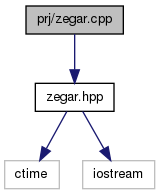
\includegraphics[width=192pt]{zegar_8cpp__incl}
\end{center}
\end{figure}


\subsection{Opis szczegółowy}
Definicja metody Start. Definicja metody Wynik.

Definicja metody Koniec.

Metoda, ktora powoduje start zegara.

Metoda, ktora powoduje stop zegara i oblicza czas.

Metoda, ktora wyswietla wynik. 

Definicja w pliku \hyperlink{zegar_8cpp_source}{zegar.\-cpp}.


\hypertarget{zegar_8hpp}{\section{Dokumentacja pliku prj/zegar.hpp}
\label{zegar_8hpp}\index{prj/zegar.\-hpp@{prj/zegar.\-hpp}}
}


Definicja klasy \hyperlink{class_tablica}{Tablica}.  


{\ttfamily \#include $<$ctime$>$}\\*
{\ttfamily \#include $<$iostream$>$}\\*
Wykres zależności załączania dla zegar.\-hpp\-:
\nopagebreak
\begin{figure}[H]
\begin{center}
\leavevmode
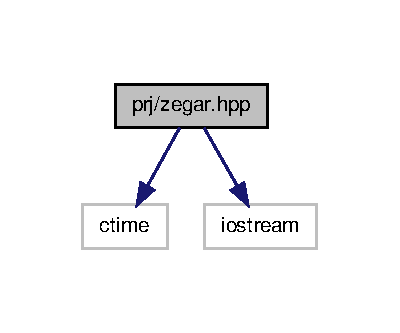
\includegraphics[width=192pt]{zegar_8hpp__incl}
\end{center}
\end{figure}
Ten wykres pokazuje, które pliki bezpośrednio lub pośrednio załączają ten plik\-:
\nopagebreak
\begin{figure}[H]
\begin{center}
\leavevmode
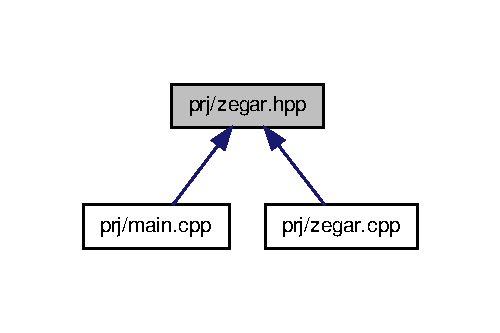
\includegraphics[width=240pt]{zegar_8hpp__dep__incl}
\end{center}
\end{figure}
\subsection*{Komponenty}
\begin{DoxyCompactItemize}
\item 
class \hyperlink{class_zegar}{Zegar}
\end{DoxyCompactItemize}


\subsection{Opis szczegółowy}
Definicja klasy \hyperlink{class_tablica}{Tablica}. Klasa odpowiadaj�ca za operacje wykonujace sie na tablicy takie jak\-: zamienienie elementow, odwrocenie tablicy, dodanie elementu, dodanie elementow, operator + operator, operato == 
\begin{DoxyParams}[1]{Parametry}
\mbox{\tt in}  & {\em clock\-\_\-t} & start, koniec -\/ zmienne przechowuja aktualny czas systemu \\
\hline
\mbox{\tt in}  & {\em czas} & -\/ przechowuje roznice czasow koniec i start \\
\hline
\end{DoxyParams}


Definicja w pliku \hyperlink{zegar_8hpp_source}{zegar.\-hpp}.


%--- End generated contents ---

% Index
\newpage
\phantomsection
\addcontentsline{toc}{chapter}{Index}
\printindex

\end{document}
